%#! platex UserGuideJa
\chapter{はじめに}
\label{chap:1}
本ガイドは,Open Source Field Operation and Manipulation
(OpenFOAM) C++ライブラリ,バージョン2.0.0リリースに付属するものです.
本ガイドでは,まず\autoref{chap:2}のチュートリアル演習を通して,
またそれ以降はOpenFOAMを構成する
個々のコンポーネントに関するより詳細な記述によって,
OpenFOAMの基礎的な操作法に関して説明しています.

OpenFOAMに関して最も重要なことは,
主にアプリケーションとよばれる実行ファイルを作成するために使われる
C++ライブラリであるということです.このアプリケーションは,
連続体力学における特定の問題を解くためのソルバ,
およびデータに対する各種の操作を行うためのユーティリティの
二つのカテゴリに大別されます.
OpenFOAMの配布物は\autoref{chap:3}に述べるように,
多岐にわたる問題を扱うための多数のソルバおよびユーティリティを含んでいます.

OpenFOAMの特長の一つは,背景となる手法,物理学,
関連するプログラミング技術に関する知識があれば,
新しいソルバやユーティリティをユーザ自身が作成可能であることです.
これらに関する情報はプログラマズ・ガイドに掲載しています.

OpenFOAMには前処理・後処理の環境も含まれています.
前処理・後処理へのインタフェースもまたOpenFOAMの
ユーティリティですから,OpenFOAM内の全ての環境にわたって
データの取扱いの一貫性が保たれています.
OpenFOAMの全体的な構造を\autoref{fig:1.1}に示します.


\begin{figure}[ht]
 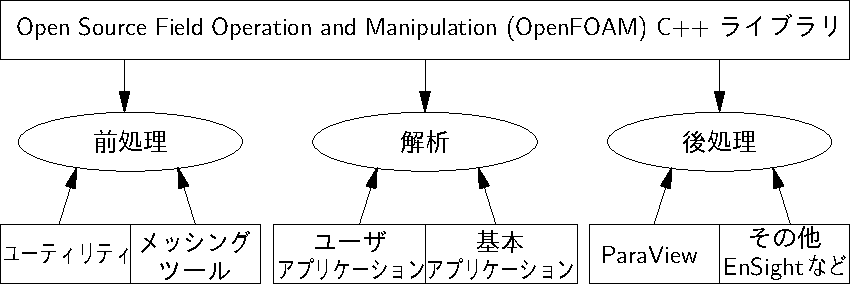
\includegraphics{fig-1-1}
 \caption{OpenFOAMの全体的な構造}
 \label{fig:1.1}
\end{figure}


前処理やOpenFOAMのケースの実行方法については,\autoref{chap:4}で説明します.
\autoref{chap:5}では,
OpenFOAMに付属するメッシュ・ジェネレータを使ってメッシュを生成する方法や,
サードパーティ製品で生成したメッシュを変換する方法も説明します.
後処理については\autoref{chap:6}で説明します.

